% pandoc-xnos: cleveref fakery
\newcommand{\plusnamesingular}{}
\newcommand{\starnamesingular}{}
\newcommand{\xrefname}[1]{\protect\renewcommand{\plusnamesingular}{#1}}
\newcommand{\Xrefname}[1]{\protect\renewcommand{\starnamesingular}{#1}}
\providecommand{\cref}{\plusnamesingular~\ref}
\providecommand{\Cref}{\starnamesingular~\ref}
\providecommand{\crefformat}[2]{}
\providecommand{\Crefformat}[2]{}

% pandoc-xnos: cleveref formatting
\crefformat{equation}{Eq.~#2#1#3}
\Crefformat{equation}{Equation~#2#1#3}

\section{Observational Cosmology
Primer}\label{observational-cosmology-primer}

\subsection{Doppler Effect}\label{doppler-effect}

\subsubsection{Classical Doppler Effect}\label{classical-doppler-effect}

Suppose you are standing on the sidewalk and along the road a parked
ambulance turns on its siren. As the ambulance siren blares, it
approaches you and you notice that the pitch of the siren seems to have
increased such that it sounds higher than it did previously. Then, as
the ambulance passes and recedes behind you another change occurs, but
now the pitch seems to have decreased such that it sounds much deeper
than before. This is a classic example of the phenomenon known as the
\emph{Doppler effect} where a stationary observer experiences a change
in frequency due to a moving wave source. More precisely, the Doppler
effect produces an observed shift in the original wave emitted such that
an approaching wave source (i.e.~the ambulance moving towards the
observer) will seemingly appear to have an increase in frequency,
meanwhile a receding wave source (i.e.~the ambulance moving away from
the observer) will appear to have a decrease in frequency. However, it
is important to keep in mind that while a shift is observed, in
actuality there are no changes to the emitted wave or the wave source
itself. The relationship for the \emph{Doppler shifted} frequency
observed is given by the expression:

\begin{equation}f_\text{obs} = f_\text{em} \left (\frac{v_\text{wave} + v_\text{receiver}}{v_\text{wave} + v_\text{source}}  \right )\label{eq:classicdop}\end{equation}

\noindent where \(f_\text{obs}\) describes the observed Doppler shifted
frequency, \(f_\text{em}\) is the emitted frequency by the wave source,
\(v_\text{wave}\) is the speed of the emitted wave and is defined by
wave velocity equation as the wavelength \(\lambda_\text{em}\) times the
frequency \(f_\text{em}\), \(v_\text{receiver}\) is the velocity of the
observer receiving the signal (positive when moving towards the source
and negative in the opposite direction), \(v_\text{source}\) is the
velocity of the moving wave source emitting the signal (positive when
receding from the observer and negative in the opposite
direction)\footnote{As you may have noticed, the relationship results in a constant Doppler shift in the frequency which is not what you would actually observe when an ambulance passes by. The increasing and decreasing in frequency is actually a product of the ambulance passing parallel to the observer which results in a changing angle between the moving wave source and the line of sight between the ambulance and the observer such that $v_{_\text{LOS}} = v_\text{source} \cdot \text{cos}\ \theta$. However, if the ambulance were to drive directly at the observer, they would would hear a constant increase or decrease in the frequency as is the case in our example.}.

From \xrefname{Eq.}\cref{eq:classicdop}, we can see that for an
approaching ambulance for which the observer is at rest:
\(v_\text{receiver} = 0\), \(v_\text{source}\) is negative indicating
the ambulance is moving towards the observer, and \(v_\text{wave}\) is
the speed of sound at approximately \SI{340}{m/s}. Given these
conditions, we can write the Doppler effect for sound observed by a
stationary observer (as in our ambulance example) as

\begin{equation}f_\text{obs} = f_\text{em} \left (\frac{1}{1 -v_\text{source} / v_\text{wave}}  \right )\label{eq:ambdop}\end{equation}

\noindent where we have simplified the equation in terms of the ratio of
the source velocity to the speed of the wave.

\subsubsection{Relativistic Doppler
Effect}\label{relativistic-doppler-effect}

While the Doppler shifted sound waves experienced by an observer can
accurately be described by \xrefname{Eq.}\cref{eq:classicdop} and
\xrefname{Eq.}\cref{eq:ambdop}, this form of the equation is only true
for wave sources that move much slower than the speed of light. For
electromagnetic waves (such as visible light) special relativity
dictates that the relationship must be altered such that Lorentz
symmetry\footnote{Lorentz symmetry states simply that the laws of physics must uphold in any reference frame.}
is upheld. Therefore, the relativistic form of the Doppler effect
becomes

\begin{equation}\nu_\text{obs} = \nu_{em}\ \sqrt{\frac{1- \beta}{1 + \beta}}\label{eq:reldop}\end{equation}

\noindent where \(\nu\) is the relativistic notation for frequency
(equivalent to \(f\) in the classical case) and the dimensionless
\(\beta = v/c\) is ratio between the relative velocity
\(v = v_\text{source} - v_\text{rec}\) to the speed of light \(c\). Note
that \(\beta\) is positive when the observer and the source are receding
away from each other and negative when the observer and the source are
approaching each other---analogous to \(v_\text{source}\) in the
classical case. The relativistic Doppler effect may seem quite different
from our classical case in \xrefname{Eq.}\cref{eq:classicdop}; however,
if we Taylor expand about the low-velocity limit (for \(v \ll c\)) where
the relative velocity is much slower than the speed of light we find
that
\(\nu_\text{obs} = \nu_\text{em} \left( 1 - \beta + \mathcal{O}(\beta^2) \right)\).
Using the same low-velocity analysis on
\xrefname{Eq.}\cref{eq:classicdop}, we find that
\(f_\text{obs} = f_\text{em} \left( 1 - \beta \right)\) such that the
relativistic Doppler effect reduces to the classical case for relative
velocities much less than the speed of light.

\subsubsection{Redshift}\label{redshift}

The Doppler effect is particularly useful in astronomy because each
element has a unique spectrum of emission and absorption lines that will
appear Doppler shifted by a moving astronomical source. Astronomers may
draw useful information from Doppler shifts in spectroscopic
measurements, such as the distance, velocity, and composition of an
astronomical object. This is accomplished by comparing the position of
the spectral lines of a specified element against their rest frame
wavelength. We will find it useful to define the relativistic Doppler
shift in terms of the redshift \(z\) of the initial signal as

\begin{equation}z \equiv \frac{ \lambda_\text{obs}}{\lambda_\text{em}} - 1 =  \frac{\Delta\lambda}{\lambda_\text{em}} = \sqrt{\frac{1 + \beta}{1-\beta}} - 1\label{eq:redshift}\end{equation}

\noindent where we have used the wave velocity relation to rewrite the
Doppler shift in \xrefname{Eq.}\cref{eq:reldop} in terms of wavelength.
The term redshift is used because it implies that the signal's
wavelength has been lengthened, synonymous to longer wavelengths in the
visible spectrum corresponds to red light. Likewise, a negative redshift
is equivalent to a blueshift, a shortening of the signal's wavelength.
From the limiting case for the low-velocity regime where \(v \ll c\),
using our previous result in \xrefname{Eq.}\cref{eq:redshift} we find
that

\begin{equation}z \simeq \frac{v}{c}\label{eq:lowvelocity}\end{equation}

\noindent where receding sources appear redshifted and approaching
sources appear blueshifted relative to an observer.

\subsection{Standard Candles}\label{standard-candles}

A Standard candle is a class of astronomical objects that possess an
intrinsic quality shared amongst the class, a `standard' so to speak,
that provides a well known luminosity. Examples of standard candles
include Cepheid variable stars, planetary nebula, Tully-Fisher relation
for spiral galaxies, and supernovae amongst others. All of these
contribute to the cosmic distance ladder, a chain of various techniques
used to measure different length scales.

\subsubsection{Parallax}\label{parallax}

The foundation of the distance ladder is the geometric effect of
measuring nearby astronomical objects called parallax. The parallax uses
the apparent displacement of a distant object as the observer changes
their position to measure the distance and is described by \(d = 1 / p\)
(for \(p \ll 1\, \text{radian}\)), where \(d\) is the distance in
parsecs (\SI{1}{\parsec} \(\simeq\) \SI{3.26}{\lightyear}) and \(p\) is
the parallax angle in arcseconds. While this method provides some of the
most accurate distance measurements, it is limited by the apparent
displacement which for large distances becomes difficult to
resolve\textbackslash{}footnote\{Parallax measurements from ground-based
telescopes are able to resolve to distances of about
\SIrange{50}{100}{\parsec}, while space-based telescopes are able to
extend this limitation to \SIrange{200}{300}{\parsec} within 10\%
accuracy.\}.

\subsubsection{Cepheid Variable Stars \& The Magnitude
System}\label{cepheid-variable-stars-the-magnitude-system}

Despite the limitations of the parallax, the accuracy of the method
allows astronomers to calibrate other methods that can measure distances
at much greater length scales on the cosmic distance ladder. Cepheid
variables are stars that undergo a period of pulsation---a defined
period of contraction and expansion---during which a change in
brightness is
observed\footnote{It should be noted that when we mention brightness we are explicitly referring to the flux of light we measure in \si{\watt\per\metre\squared}.}.
Due to the change in physical size, the absolute brightness or
\emph{luminosity} of the Cepheid changes such that we observe a change
in apparent brightness on Earth. What makes Cepheid variables an
important standard candle is that not only does this intrinsic quality
holds amongst the class, but more importantly, from empirical evidence
we know that there is a direct relationship between the period of
pulsation and the true luminosity of Cepheids: unsurprisingly, we call
this the \emph{period--luminosity relationship}. Distance measurements
are normally a challenge to calculate due to the required luminosity as
defined by the inverse square law for light:

\begin{equation}B= \frac{L}{4 \pi \cdot d^2}\label{eq:invsqrlaw}\end{equation}

\noindent where \(d\) is the distance, \(L\) is the luminosity, and
\(B\) is the apparent brightness as measured on Earth. But, by measuring
the period of pulsation from changes in apparent brightness we are able
to determine the luminosity and thus measure distance to Cepheids in
galaxies far greater than the reach of parallax measurements. The
accuracy of the period--luminosity relationship is dependent, however,
on standard luminosity measurement to nearby Cepheids in which the
parallax distance can be used to calibrate the method. For example, in
2002 the Hubble Space Telescope in partnership with the Hipparchus
Satellite was able to use the parallax method to determine the most
accurate distance measurement to the closest known Cepheid variable
star, Delta Cephei, thus establishing a cosmic benchmark on the ladder
for other distance methods. The period--luminosity relationship is often
regarded as the stepping stone by which other methods are compared
against to improve the accuracy of our distance measurements.

A more common astronomical method of measuring distance analogous to the
inverse square law of light in \xrefname{Eq.}\cref{eq:invsqrlaw}
involves the magnitude system, a logarithmic magnitude scale of a
stellar object's
brightness\footnote{invented by the Greek astronomer Hipparchus and Ptolemy. Eye sees logarithmically. Makes sense!}.
Due to the logarithmic nature, the system is fairly counterintuitive
such that an object brightness are given in `reverse order' whereby
brighter objects have a negative magnitude while dimmer objects have a
positive magnitude. We define the apparent magnitude \(m\) (as seen from
Earth) as

\begin{equation}m \equiv m_a - m_b = -2.5 \log_{10} \left( \frac{B_a}{B_b} \right)\label{eq:mag}\end{equation}

\noindent where \(m_a\) is the magnitude of object of interest and
\(m_b\) is of a comparison object and \(B_a\) and \(B_b\) correspond to
their respective apparent brightness as defined in
\xrefname{Eq.}\cref{eq:invsqrlaw}.

From \xrefname{Eq.}\cref{eq:mag} it is clear that a change of 1
magnitude corresponds to a 2.5 decrease in brightness between the
objects. In order to standardize the relative comparison of magnitudes
we define \(m_b\) to be the apparent brightness of the star Vega such
that objects that are brighter have a negative magnitude and objects
that are dimmer have a positive
magnitude\footnote{By this standard, it would naturally follow that Vega has a reference magnitude of 0}.
We can measure the luminosity of an object in the magnitude system
through the absolute magnitude \(M\) by expressing
\xrefname{Eq.}\cref{eq:mag} in terms of the inverse square law such that

\begin{equation}M = m - 2.5 \log_{10} \left[ \left( \frac{d}{10\, \text{pc}} \right)^2 \right] \label{eq:absmag}\end{equation}

\noindent where \(m\) is the apparent magnitude and \(d\) is the
distance in
parsecs\footnote{The convention assumed here is to measure the absolute magnitude of an astronomical object at a standard astronomical distance of 10\si{\parsec}}.
Finally, we can express \xrefname{Eq.}\cref{eq:absmag} in terms of the
distance modulus \(\mu = m - M\), the difference between the apparent
magnitude \(m\) and the absolute magnitude \(M\), such that

\begin{equation}\mu \equiv m - M = -5 + 5  \log_{10} (d) + K.\label{eq:distmod}\end{equation}

\noindent where the \(K\) correction term is non-zero if
\(d\gg\)\SI{10}{\parsec} due to extinction by gas and dust.

\subsubsection{Tully-Fisher Relationship \& Fundamental
Plane}\label{tully-fisher-relationship-fundamental-plane}

Building off the stepping stone of the Cepheid' period--luminosity
relationship, we can use the Tully-Fisher relation and Fundamental plane
to extend the distance ladder to scales on the order of
1\si{\Gigaparsec}---the length scales of galaxy clusters.

The Tully-Fisher relation is an empirically driven relationship between
the rotational velocity of a galaxy and its absolute magnitude. In the
context of the distance ladder it forms one of the most important
distance estimators due to its measurement of the 21-centimeter hydrogen
line, a far infrared line in the microwave spectrum, which is relatively
unperturbed by objects that normally are opaque to shorter
wavelengths\footnote{This technique is especially important to physical cosmology for its accurate prediction of the ratio of luminous matter in the galaxy disk to the dark matter halo that surrounds it. For further reading refer to Desmond et al., 2015 on the Tully-Fisher Relation and mass-size relations to halo abundance. https://arxiv.org/abs/1506.00169}.
Given the 21-centimeter hydrogen line, we can measure the redshift and
blueshift due to the rotation of a galaxy and estimate the rotational
velocity of the galaxy.

However, given that we need distance estimates to measure the luminosity
in terms of the absolute magnitude, again we can see the distance ladder
in effect in that we use Cepheid distance measurements from both
parallax and period-luminosity relationship within individual galaxies
to calibrate the distance to the galaxy themselves. Subsequently, we can
plot the rotational velocity and the absolute magnitude of individually
calibrated galaxies to show the Tully-Fisher relation. Thus, given a
rotational velocity from far redshift objects we can not only estimate
the absolute magnitude, but more importantly a distance estimate that
otherwise wouldn't be possible.

\begin{figure}
\centering
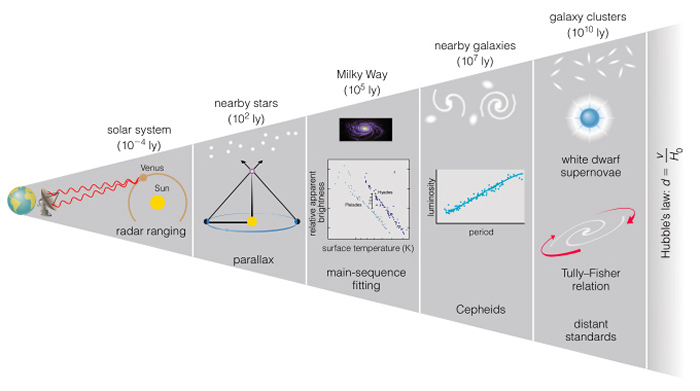
\includegraphics{http://www.daviddarling.info/images/distance_ladder.jpg}
\caption{img}
\end{figure}

As we have seen, these techniques often overlap in the length scales
they measure which is important for the calibration of the ladder
through overlapping distance measurement within individual galaxies
allowing allowing for multiple classes of distance estimators. Moreover,
from \xrefname{Eq.}\cref{eq:invsqrlaw} equation, we can see that the
accuracy of our distance estimates depends on how well we estimate the
object's true luminosity. Thus, determining the most suitable and
accurate standard candles is the trickiest aspect of distance
measurements as each method introduces some form of uncertainty.
Regardless of the challenges in the method, distance measurements are
one of the only methods that allow us to probe the cosmos and test our
theories of the Universe. From this perspective, we see that distance
measurement truly provide the foundation for understanding the structure
and evolution of the universe---the \emph{cosmology} of our universe.

\subsection{Hubble's Law}\label{hubbles-law}

In the late 1920s using distance and spectroscopic redshift measurements
of Cepheid variables, Edwin Hubble found that a galaxy's relative
velocity away from Earth is proportional to the distance between us. The
relationship now known as Hubble's law can be expressed as

\begin{equation}v \simeq cz = H_0 d\label{eq:Hubble}\end{equation}

\noindent where we have expressed the relative velocity \(v\) (in
\si{km/s}) in terms of the low-velocity limit from
\xrefname{Eq.}\cref{eq:lowvelocity}, \(H_0\) is the proportionality
constant between the relative velocity and the distance to the object in
\si{\km\per\s\per\Mpc}, and \(d\) is the distance in megaparsecs
(\SI{e6}{\parsec} \(=\) \SI{1}{\Mpc}). The proportionality constant
\(H_0\) is better known as the Hubble constant, but is most usefully
written as \(H_0= 100\, h\,\)\si{\km\per\s\per\Mpc} where \(h\) is the
dimensionless Hubble parameter defined by the current accepted value.

\begin{figure}
\centering
\includegraphics{https://cdn-images-1.medium.com/max/1000/1*ZmaIxrEA2RsueTvaGMOg3Q.jpeg}
\caption{img}
\end{figure}

While the redshift observed on Earth is often interpreted as a Doppler
shift due to the method of measurement, this leads to a troubling
interpretation of the Universe. That being that if the relative velocity
is due to a Doppler redshift, than this would imply that everything in
the night sky is receding away from us and that the Earth is located in
a privileged place in the Universe. However, as Hubble amongst others
had noticed, this statement is in obvious conflict with the Copernican
principle which states that humans are not privileged observers of the
Cosmos---i.e.~that we are not located anywhere special with regards to
the Universe around us. Another possible interpretation that does not
require sacrificing the Copernican principle had been proposed
independently as part of solutions to Einstein's field equation for
general relativity by the Soviet mathematician Alexander Friedmann and
the French astronomer Georges Lamaitre: that we reside in an expanding
universe and Hubble's law provided the first empirical evidence
supporting this theory. Under this interpretation, the relative velocity
is not a result of intrinsic motion of galaxies away from us, but rather
the result of the space between us stretching.

Moreover, Hubble's law not only implies that the Universe is expanding,
but that it is doing so at an accelerating rate. The Hubble constant is
currently measured in the range of
\SI{67-75}{\km\per\s\per\Mpc}\footnote{Add footnote on discrepancies between Planck Satellite and Supernovae Type Ia measurements},
meaning that every megaparsec of space is being stretched at a rate of
approximately \SI{70}{\km\per\s}.

\begin{figure}
\centering
\includegraphics{https://www.astro.rug.nl/~weygaert/tim1publicpic/dtfe/2dFpanel.dtfe.lres.gif}
\caption{img}
\end{figure}

\subsection{Peculiar Velocity}\label{peculiar-velocity}

Hubble's law represents an empirical relationship for the expanding
universe where each galaxy is static with respect to cosmological
expansion. Given \xrefname{Eq.}\cref{eq:Hubble} we can estimate the
cosmological redshift \(z_\text{cos}\) due to expansion from
\(z_\text{cos} \equiv H_0 d/c\). However, an ideal Hubble's law neglects
gravitational attraction to higher density regions of space which induce
`peculiar' motion that deviates from cosmological expansion velocity
\(H_0d\) known as the Hubble flow. The consequence of a continuous
inflow of matter towards these regions of space is a state of
over-density known as gravitational collapse, which provides the means
for the formation and growth of structure in the local Universe. Thus,
measurements of peculiar velocity are a compelling cosmological probe of
local structure due to the motion of galaxies tracing the underlying
density field.

We can estimate peculiar velocities as deviations within the observed
redshift \(z_{obs}\) from Hubble's law as a result of Doppler redshift
\(z_\text{doppler}\) due to local motion. Unfortunately we are
observationally limited to receding and approaching wavelengths along
the 1D line-of-sight component of a galaxy's full 3D peculiar velocity
vector. Any transverse motion along the line-of-sight is far too small
to be detected through spectroscopic measurements and thus we would also
expect any contribution to the line-of-sight to be in the form of noise
in the signal. Following \xrefname{Eq.}\cref{eq:Hubble}, at low-redshift
where \(v \ll c\), the line-of-sight component of the peculiar velocity
\(v_p\) is given by the familiar form

\begin{equation}v_p \approx cz_\text{obs} - H_0d\label{eq:pecveloapprox}\end{equation}

\noindent where \(c\) is the speed of light, \(z_\text{obs}\) is the
observed redshift, and \(H_0d\) is the cosmological expansion velocity
at a given comoving
distance\footnote{Comoving distance refers to the real distance between two objects at rest with respect to the Hubble flow. In simpler terms, comoving distance is the physical distance between two objects in the absence of cosmic expansion.}
\(d\)\footnote{Davis et al shows that due to redshift not being an additive property this crude approximation is only accurate for $z_\text{obs} << 0.1$, but for the introductory purposes of this section we find this form more than sufficient. We will revisit this equation in Section 2.#}.
Therefore given a distance indicator, the comoving distance \(d\) can be
measured independently from the observed redshift \(z_\text{obs}\)
allowing us to estimate the peculiar velocity. The most common form of
distance indicators are the various standard candles introduced in Sec
1.\# which unfortunately suffer from large uncertainties. In contrast to
the high accuracy redshift measurements available, the uncertainty on
distance estimators can be upwards of \(\simeq 20\%\) which can lead to
uncertainties in the peculiar velocity measurement on the order of the
velocity itself. Typical peculiar velocity measurement are expected to
be of order \SI{300}{km/s} while the errors scale largely with the
distance of the galaxy such that uncertainty \(\delta_{v_p}\) can be
approximated by \(\delta_{v_p} \approx 0.20 H_0 d\). Given the large
uncertainties, peculiar velocity measurements must be estimated through
statistical means thus requiring large velocity surveys with both
distance and redshift
measurements\footnote{In Section 2.# we will discuss an estimator method developed by Watkins & Feldman that provides a more accurate method of statistically estimating peculiar velocities.}.
